\documentclass[12pt]{article}
\usepackage[hmargin={1in},vmargin={1in,1in},foot={.6in}]{geometry}   
\geometry{letterpaper}              
\usepackage{color,graphicx}
\usepackage{setspace}
\usepackage{amsmath}
\usepackage{amssymb}
\usepackage{varioref}
\usepackage{textcomp}
\usepackage{textcomp}
\usepackage{mflogo}
\usepackage{wasysym}
\usepackage[normalem]{ulem}
\usepackage{hyperref}

\newcommand{\HRule}{\rule{\linewidth}{0.25mm}}

\usepackage{fancyhdr} % This should be set AFTER setting up the page geometry
\pagestyle{plain} % options: empty , plain , fancy
\lhead{}\chead{}\rhead{}
\renewcommand{\headrulewidth}{.5pt}
\lfoot{}\cfoot{\thepage}\rfoot{}
\newcommand{\txtp}{\textipa}
\renewcommand{\rm}{\textrm}
\newcommand{\sem}[1]{\mbox{$[\![$#1$]\!]$}}
\newcommand{\lam}{$\lambda$}
\newcommand{\lan}{$\langle$}
\newcommand{\ran}{$\rangle$}
\newcommand{\type}[1]{\ensuremath{\left \langle #1 \right \rangle }}

\newcommand{\bex}{\begin{exe}}
\newcommand{\eex}{\end{exe}}
\newcommand{\bit}{\begin{itemize}}
\newcommand{\eit}{\end{itemize}}
\newcommand{\ben}{\begin{enumerate}}
\newcommand{\een}{\end{enumerate}}

\newcommand{\gcs}[1]{\textcolor{blue}{[gcs: #1]}}
\definecolor{Green}{RGB}{10,200,100}
\newcommand{\ndg}[1]{\textcolor{Green}{[ndg: #1]}}
\newcommand{\jd}[1]{\textcolor{red}{[jd: #1]}}

\thispagestyle{plain}

\begin{document}

{\flushright

\vspace{25pt}
%Gregory Scontras\\
%Judith Degen\\
%Noah D.~Goodman\\
%Department of Psychology\\
%Stanford University\\
%Stanford, CA 94305\\[20pt]

\noindent June 9, 2016\\[25pt]}


\noindent Dear Editor,\\

\noindent We would like to thank you and the three anonymous reviewers for your helpful comments on our paper, ``Subjectivity predicts adjective ordering preferences.'' As you will recall, you highlighted the following three concerns: 

\ben

\item \emph{The discussion/framing of other approaches needs some attention: R1 mentions some other hypotheses that deserve discussion, and R2 takes issue with the framing of previous approaches as syntactic vs semantic. This latter point is related to another issue mentioned by R2 and R3: the distinction between online decisions about adjective ordering versus conventionalized ones. Clarifying how your proposal relates to these questions would, I think, help address these concerns.}

We have included reference to and discussion of the other hypotheses that the reviewers mention. We have also taken care in our framing to distinguish the \emph{conventionalization} of ordering preferences from the \emph{explanation} of the observed orderings; it is the latter that we investigate in our paper. Finally, we have also revised our language to emphasize that the subjectivity hypothesis is meant to synthesize---not supplant---previous approaches to adjective ordering.

\item \emph{All three reviewers express some dissatisfaction about the lack of direct comparison between your hypothesis and others. As they point out, the fact that your data are well explained by subjectivity tells us little about whether this hypothesis provides a better explanation than any other. Some of the other hypotheses may seem difficult to operationalize, but on the face of it, so is subjectivity. A quantitative comparison to other approaches would considerably strengthen the paper.}

We agree that a quantitative comparison will strengthen our claims regarding subjectivity by demonstrating not only the absolute, but also the \emph{relative} success of our hypothesis. For this reason, we ran four additional experiments and performed a host of analyses to operationalize three alternative accounts of adjective order and compare their predictions with those made by subjectivity. To satisfy journal length length requirements, we followed your suggestion and included this information in a supplement (\emph{Supporting information: Comparing subjectivity with alternative accounts of adjective order}), summarizing the results in the paper's General Discussion.
%\ndg{and summarize the results in section XX}. 
The new results demonstrate the robust replicability of the success of subjectivity in predicting adjective order. They also demonstrate that the alternative accounts we considered add little to our understanding of ordering preferences: subjectivity is a better predictor. %while the alternatives did not add explanatory value, with the exception of inter/subsectivity \jd{this is true, right?}. 
This exploration has led us to appreciate the intuitive appeal of the subjectivity hypothesis, which targets an easily-accessed, stable psychological construct: adjective subjectivity.


\item \emph{R1 and R2 both express confusion/skepticism about the explanation for *why* subjectivity should determine ordering. I suspect that some readers will be skeptical regardless of the explanation, but it would be good to clarify if possible -- or alternatively to admit that the hypothesis is based purely on descriptive adequacy and indeed it is not clear why it holds. (If so, this might suggest that subjectivity is correlated with some other, perhaps as yet undetermined, factor that could provide a more convincing mechanism for ordering.)}

Reviewers 1 and 2 were uncomfortable with the paper's concluding paragraph, presumably because they took our speculation as a claim about the psychological mechanism. In our revision, we have modified our language to emphasize that these musings are indeed just speculation and suggestions for future research, informed by our experimental results. While we do not claim to have a theoretical explanation for why subjectivity should predict ordering preferences, we do not believe this decreases the significance of the finding. 
(An extraordinarily high correlation between two \emph{a priori} unrelated but theoretically interesting behavioral measures is itself an important finding.) 
%In this case, we believe it is one that will serve as a call for new theoretical work. We offer a suggestion for a direction to pursue---the consolidation of highly-informative content around the noun---while acknowledging that the explanation may turn out to be something completely different. 

\een


In the remainder of this letter, we consider in more detail each of the reviewers' concerns.


\newpage

\subsubsection*{Reviewer 1:}

\ben

\item \emph{I really appreciate the historical framing of the literature, but I do miss some very influential semantic or `psychological' contemporary hypotheses: The hypothesis that not subjectivity, but subsectivity, determines adjective order (Trueswell 2009); the apparentness hypothesis (Sproat \& Shih, 1991); even Laenzlinger (2005). Ignoring these literatures make it seem like the authors are uncomfortable with the idea that
others had the same intuition they had, which they shouldn't be. It does, however, relativize the present findings: Subjectivity is one
explanation for a whole range of factors that determine adjective order; and as it stands, I am not convinced that subjectivity explains the data any better than the subsective/intersective distinction, or apparentness. All these concepts overlap significantly, and if I am to buy the explanation of subjectivity, I want at the very least some additional data that allow a comparison.}

We have added the suggested references, and clarified our language to stress that subjectivity synthesizes rather than supplants the work that precedes ours (cf.~our response to the Editor's point 1). To address the issue of comparing the predictions of subjectivity with those made by previous hypotheses, we have added the \emph{Supporting information: Comparing subjectivity with alternative accounts of adjective order} (cf.~our response to the Editor's point 2).

\item \emph{I am a little bit confused about Experiment 2. If I understand correctly (and I might not!), this study is the same as Experiment 1, but with a wider range of adjectives. Also, the model explains the data much, much less well (88\% in Experiment 1 vs. 61\% in Experiment 2). Thus, it seems like subjectivity is no better than most models that exist; and certainly worse than Wulff (2003).}

Expt.~2 uses the same design as Expt.~1 with a much larger set of materials: 78 adjectives and 166 nouns. Many of these adjectives and most of the nouns have been ignored in previous accounts of adjective order. That subjectivity accounts for less variance in Expt.~2 is a direct result of the fact that there is \emph{more} variance in the data, owing to the massive increase in materials. Despite the decrease in predictive power from Expt.~1 to Expt.~2, subjectivity continues to perform remarkably well. As for other models (which we operationalized to the best of our abilities in order to derive comparable predictions), our new SI serves to demonstrate that subjectivity is \emph{much} better at predicting ordering preferences (see Supplement). 

It is impossible to compare the correlations we report directly with the performance of Wulff's LDA model. Wulff uses eight factors to predict a binary outcome: the relative position of two adjectives in a corpus. We used a single factor, subjectivity, to predict a gradient outcome: the strength of the preference for placing that adjective first in a multi-adjective string.
(Which is not to say that further exploration of classifier-based models is not warranted.) 
%\ndg{how does this model work? is it really incompareable?}
	
\item \emph{The hypothesis that complex concept formation is involved to a significant degree cannot be ruled out, because the set of AAN-combinations in Experiment 1 is limited, and this hypothesis was not tested in Experiment 2.}

We agree that the set of AAN-combinations in Expt.~1 was limited, which is why we in fact did test the concept-formability hypothesis in Expt.~2: in both cases, we failed to find any evidence that ordering preferences depend on the modified noun. However, we also found the concept-formability hypotheses intuitively appealing, so we followed up on this result by replicating our naturalness rating experiment with a new set of nouns chosen to maximize the probability of by-noun effects.
Complex concepts will be described using the two-word name, presumably yielding more occurrences of this bigram than would be expected from the unigram frequencies of the noun and adjective.
We thus chose new nouns whose co-occurrence probability with our 26 adjectives in the BNC is far greater than one would predict on the basis of their individual word probabilities. 
We used these new materials in a direct replication of our naturalness ratings experiment, and performed the same nested model comparison predicting naturalness ratings either by \textsc{adjective} only, or by \textsc{adjective} together with its interaction with \textsc{noun}. The model comparison revealed that noun-specific ratings did not explain any additional variance in ordering preference beyond adjective-level ratings. However, adjective subjectivity scores (obtained in \emph{Expt 1.2 Subjectivity}) account for  85\% of the variance in the new naturalness ratings ($r^2${=}0.85, 95\% CI [0.64,  0.93]). Thus, while we fail to find evidence of noun-specific effects both in our original materials and in materials specifically designed to deliver such effects, we continue to see that subjectivity predicts adjective ordering preferences. We report on the details of this replication in the new supplement to our manuscript.

\item \emph{The proposed psychological mechanism for adjective order seems counterintuitive. If it was indeed the case that more subjective adjectives are ruling out miscommunications, then they should come first in post nominal positions. This is indeed the case for Romance languages, for example. However, then one would expect the same linear order in prenominal positions.}

Our speculation is that \emph{less} subjective content rules out miscommunications, which is why less subjective content appears closer to the noun in both pre- and post-nominal languages. This idea relies on a notion of hierarchical---rather than simply linear---ordering, and implicates 
%\ndg{calls into question? re-word} 
diachronic processes that likely deliver the preferences we observe today. We have added discussion of these points to the manuscript.

\item \emph{The cartographic approach does not seek adjective ordering preferences in their structure (that sounds as if there is something about their morphology that determines their order); it attempts to build a structural model.}

We agree, and we did not intend to suggest that cartographic approaches were concerned with adjective morphology. To avoid this confusion, we have clarified our language in discussing these approaches, abandoning the term ``cartographic'' altogether.

\item \emph{The idea that miscommunication increases with vague adjectives is a very relevant hypothesis to the author's model, and would be one (interesting) way of expanding the current paper.}

We agree, and have included discussion of this idea in our manuscript. However, we believe expanding the current paper with further exploration of this point would take us well beyond the scope---and word limits---of the paper. We believe these explorations are better suited to future research.

\item \emph{Table 1: Why are there different numbers of adjectives in each category? Isn't there a big danger that the effects are driven by individual items?}

There are different numbers of adjectives in each category because we initially selected adjectives that occur relatively frequently while trying to nevertheless cover as many different adjective classes as possible, resulting in unbalanced cells. As for the reviewer's question regarding the danger of outlier-driven effects: almost all of the analyses we report were conducted on the adjective level, not the adjective class level, avoiding the possibility of inducing a class-level bias via an outlier in that class. The concern is greater for the subjectivity difference score analysis: here, we predicted naturalness ratings from a difference score that was computed by subtracting adjective \emph{class} means from each other. However, there was very little variability---and thus, no outliers---among adjectives within each class, either in subjectivity or faultless disagreement scores. We demonstrate this for the 26 Expt.~1 adjectives in the following graph, which plots mean faultless disagreement and subjectivity scores:
\begin{center}
	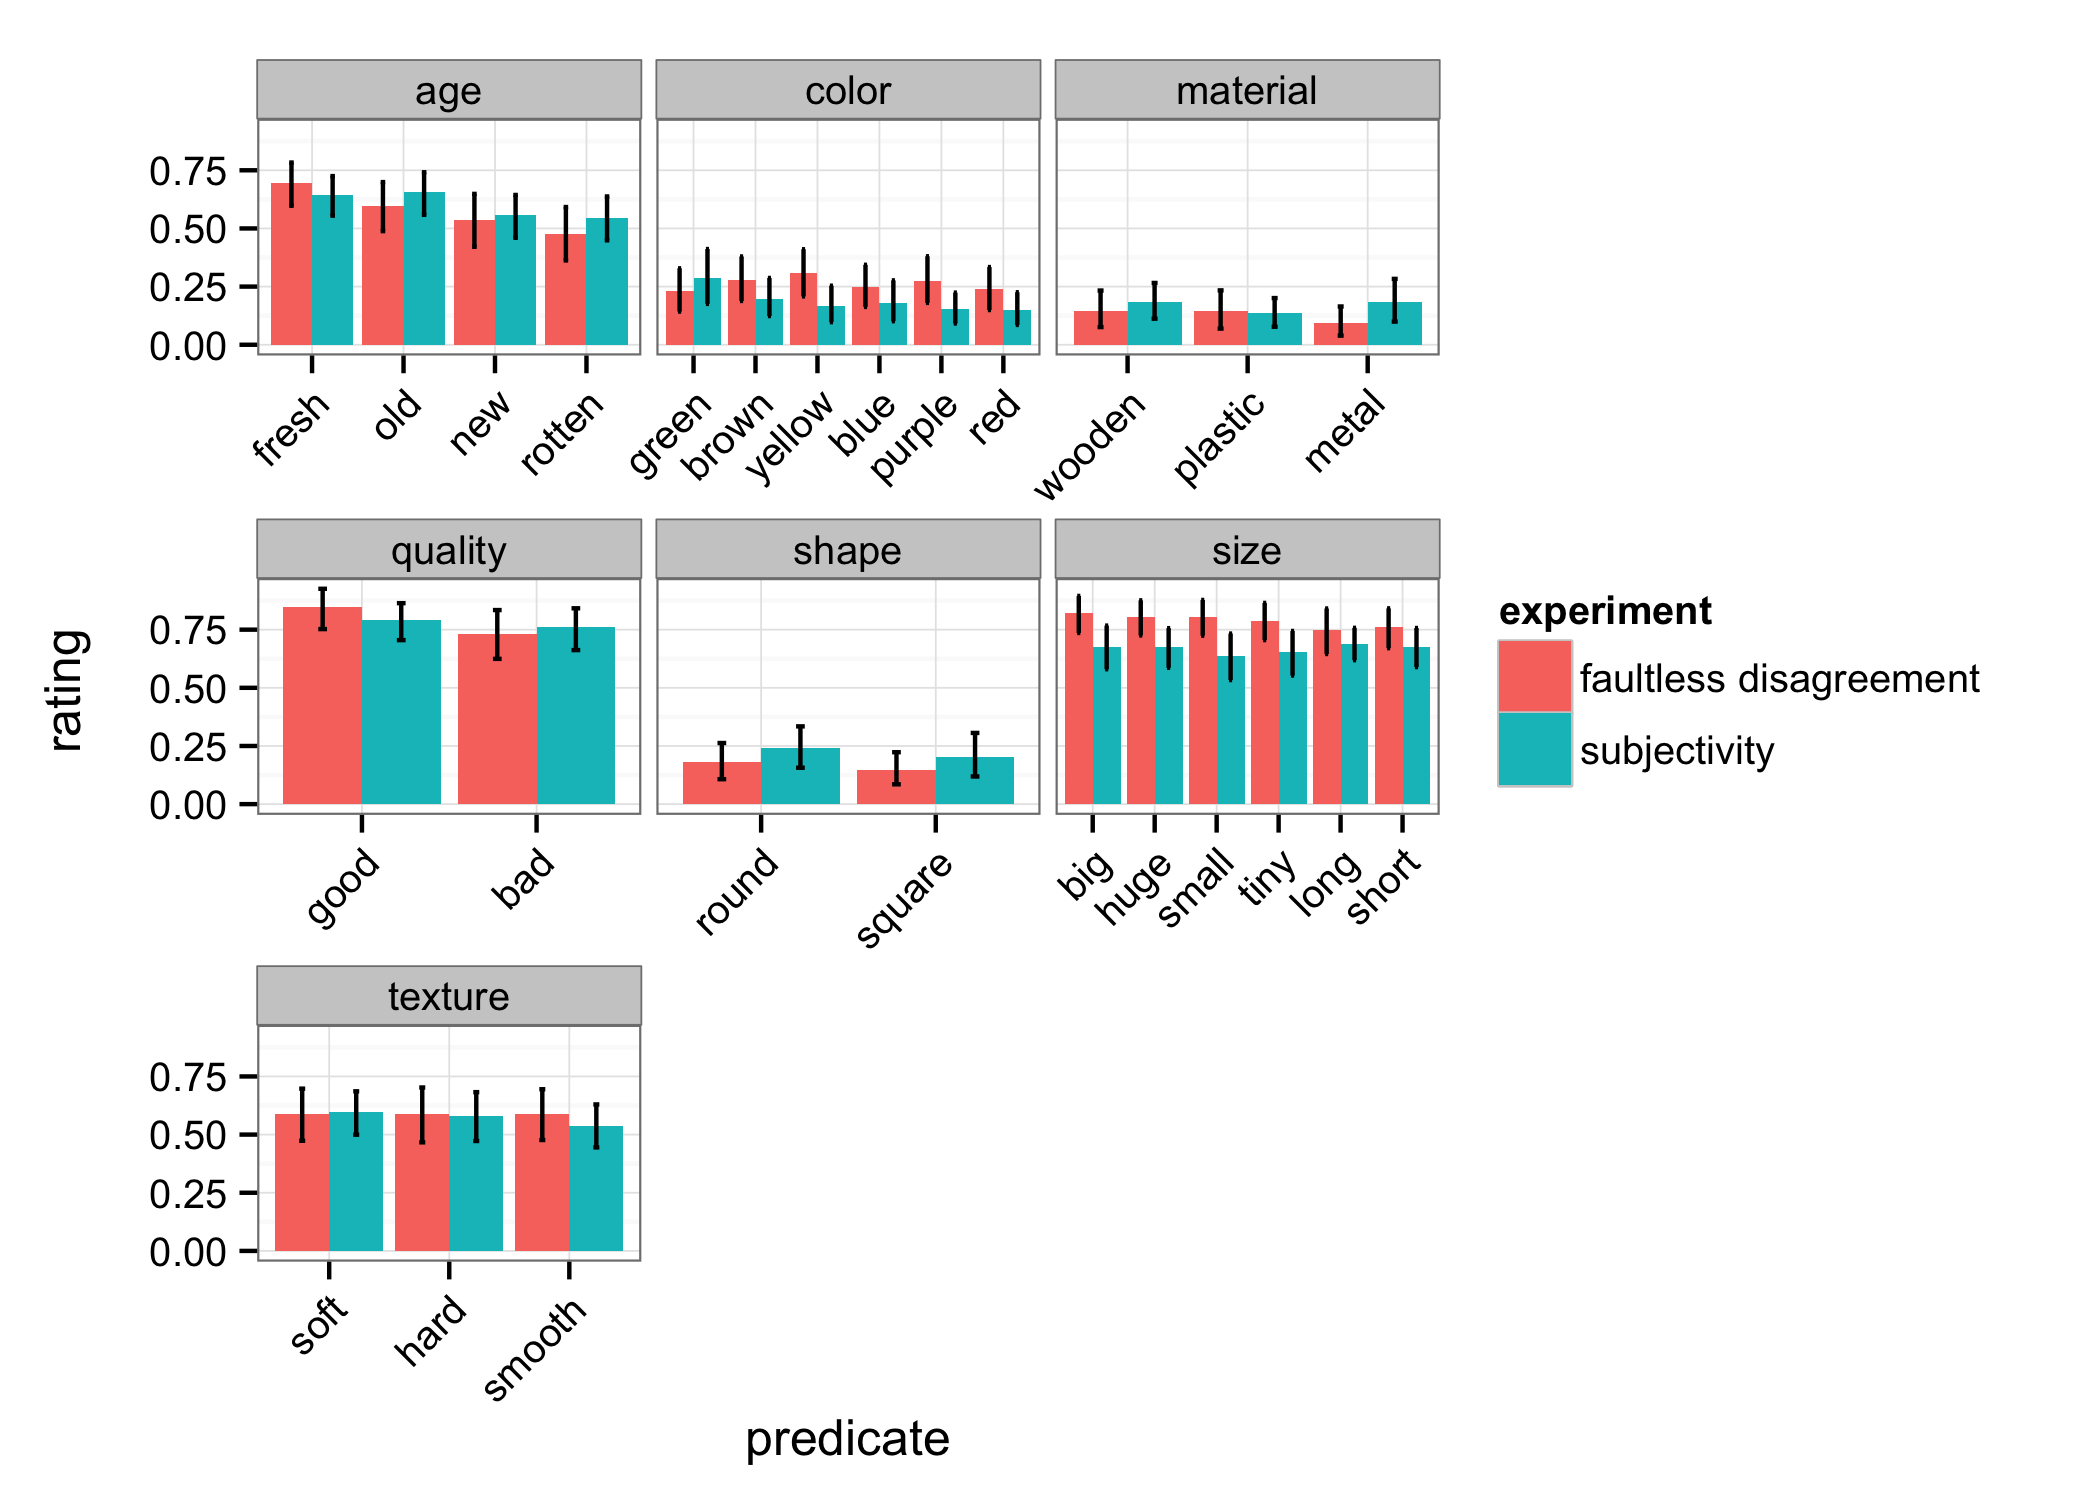
\includegraphics[width=\linewidth]{plots/pred_plot_comparison.eps}
\end{center}


\item \emph{It would be an even stronger argument for the authors if there were ordering preferences within the same semantic class, based on subjectivity.}

This is an excellent point: semantic classes serve merely to structure and smooth our data; subjectivity should apply within---as well as across---the semantic classes we test. However, we are unable to test this prediction with the current experiments. To avoid nonsensical object descriptions in our experimental items, we avoided pairing adjectives from the same semantic class, so we can't determine ordering preferences within-class.

\item \emph{(naturalness) $->$ (preference), or vice versa everywhere else}

We operationalized adjective ordering preferences as naturalness ratings for specific sequences of adjectives, which we obtained in the behavioral experiments. We believe that it is best not to conflate these two notions---naturalness ratings and the preferences they reflect.

\een



\subsubsection*{Reviewer 2:}

\ben

\item \emph{The authors suggest a number of alternative accounts of adjective ordering, for example a set of noun classes (as identified by Dixon or used by Cinque), or inherent-ness. They seem to suggest that subjectivity does a better job of operationalizing the relevant semantic notion, and indeed it does explain an impressive amount of the variance in the data. However I would find the paper *much* more convincing if the authors actually tested this by doing some model comparison.}

We followed this advice, operationalizing alternative hypotheses and comparing their predictions with those made by subjectivity. We included the additional experiments and analyses in the new \emph{Supporting information: Comparing subjectivity with alternative accounts of adjective order} (cf.~our response to the Editor's point 2 and Reviewer 1's point 1).

\item \emph{I'd like to see a bit more nuance in the presentation of the general question, in particular how previous work has explained adjective ordering based on the interaction of semantics and syntax. The authors set things up as a debate between whether syntax or semantics explains adjective ordering. But actually I think that's a conflation of two distinct (though related) questions: What is the ultimate explanation for why certain (types of) adjectives occur closer to nouns than others (across languages)? And what is the formalization/representation/conventionalization of these ordering preferences in the syntax of a language? Syntacticians like Cinque are largely interested in the latter. But that doesn't mean that they think the universal structure of the DP is unrelated to semantic features of adjectives.
I think this comes up again in the discussion/conclusion, since what the authors end up arguing for is that a particular semantic notion, subjectivity, partially determines order. But of course that leaves open the further question of how this interacts with the syntactic grammar of a language (English or otherwise). Maybe they think that the grammar encodes subjectivity along with frequency, length, etc., together these probabilistically determine order, and that's all there is to it. But it also could be that subjectivity is the ultimate source of a more deterministic set of word order rules, and the latter are encoded in the grammar. The latter seems more in line which how they introduce the issue -- there are these very systematic preferences that people show within and across languages. If subjectivity is really doing so much of the work, then it seems to me that ordering might actually be predicted to be quite flexible. In an individual instance, subjectivity will be
determined largely by context, and thus you'd imagine that certain adjectives could vary quite dramatically in their relative ordering. Is that the case? If not, then something still needs to be said about how subjectivity and conventionalized syntax interact.}

We agree that the discussion as we had it conflated why we observe the preferences we do and how the preferences are conventionalized. We have clarified our language, both in the paper's introduction and its general discussion, in order to separate these two issues. Moreover, we have stressed that it is the first question---namely, why we observe the preference we do---that we are after. We leave open this issue of how these preferences are conventionalized---settling this issue would clarify the predictions with respect to shifting contexts. However, it bears noting that the ordering preferences we observed \emph{are} quite gradient and flexible, especially from the perspective of a deterministic syntactic account (cf.~our response to Reviewer 2's point 7).

\item \emph{I'm afraid I find the explanation offered about why decreased subjectivity means closer to the noun very unconvincing. (I'm partial to the ``inherentness'' explanation myself.) Maybe the authors can elaborate, otherwise, I'm not sure what it adds.}

We have clarified our language so that what previously came across as an explanation is now clearly framed as speculation on the basis of our experimental results. We have also added to this discussion to better communicate the intuition and the directions for future work that it suggests (cf.~our response to the Editor's point 2 and Reviewer 1's point 4). As for ``inherentness'', we tested its predictions in a follow-up experiment and found that adjective inherentness---as operationalized by previous researchers---accounts for little of the variation in the ordering preferences; we included this experiment in the new \emph{Supporting information: Comparing subjectivity with alternative accounts of adjective order}.

\item \emph{``...``cartographic approach'', one could say...'' I find this an odd comment. On the one hand, Dixon was less interested in claims about syntactic structure than in understanding the semantics types of adjectives and how they are distributed across languages. On the other hand the syntactic theory that Cinque subscribes to is literally called Cartography.}

We have removed the term ``cartographic'' (cf.~our response to Reviewer 1's point 5).

\item \emph{Any comments about why noun-specific effects are not found? Along the lines of my long-winded comment (2) above, it seems like the subjectivity account might easily predict that particular adjectives might be more subjective when applied to certain nouns than others. But maybe your data just aren't able to actually show that, and with more data per noun (with different adjectives) you'd see it? Are there noun-specific differences in subjectivity ratings? Do you think they are simply ignoring the nouns in the ordering judgment task?}

We were surprised by the absence of noun-specific effects, which is why we followed up on them with new materials in a new experiment that collected more data per noun. However, once again, we failed to find evidence of noun-specific effects (cf.~our response to Reviewer 1's point 3). Our subjectivity ratings did not include noun-specific information (participants rated adjective subjectivity in isolation, without a noun). However, we followed up on our basic subjectivity experiment (\emph{Expt.~1: Subjectivity}) with a version in which participants rated the subjectivity of adjective-noun object descriptions (e.g., ``How subjective is the description `big banana'?''). There, we failed to find noun-specific differences in subjectivity ratings. However, these new subjectivity scores continue to predict the ordering preferences with remarkable accuracy ($r^2${=}0.81, 95\% CI [0.68,  0.89]; cf.~the $r^2$ value of 0.85 for the noun-less subjectivity scores). We chose not to include the null result of this new subjectivity experiment in our revision, given the brevity of the paper.

As for whether participants were simply ignoring the nouns in our ordering preference experiments, we have clear evidence suggesting that they were not. In \emph{Expt.~2: Ordering preferences} we asked participants to judge whether the adjective-adjective-noun descriptions they saw made sense. To see whether nouns had an effect on sense rates, we performed a nested linear model comparison. The models we compared predicted whether a configuration made sense either with the two \textsc{adjectives} only, or with the \textsc{adjectives} and the \textsc{noun}. The model comparison revealed that noun information does explain additional variance in sense rates beyond the two adjectives involved ($F(165,11267)=2.03, p<0.001$). We have added this analysis to the writeup of Expt.~2.


\item \emph{Can you say something more about the analyses that use adjective class configurations? Why are the subjectivity ratings sometimes better at accounting for these?}

We assume that the reviewer is referring to the difference between analyzing the data as visualized in Fig.~6 (where mean naturalness of each adjective as occurring in first position was predicted from that adjective's mean subjectivity) vs.~in Fig.~7 (where each class$_1$-class$_2$ naturalness mean was predicted from the difference in subjectivity between class$_1$ and class$_2$). The class-level difference score analysis yielded a stronger correlation between subjectivity and ordering preferences than the adjective-level one because the noise that is present in the adjective-level ratings was smoothed when collapsing across adjective classes. 


\item \emph{Can you show that adjectives that are similar in subjectivity have more flexibility in relative order when they occur together? Would be nice to have some examples of this.}

We included the configuration analyses in part to show that preferences weaken as the difference in subjectivity between two adjectives approaches zero. We now explicitly mention this point and give examples of relevant adjective pairs (e.g., ``yellow square\ldots'' and ``fresh soft\ldots'').

\een


\subsubsection*{Reviewer 3:}

\ben

\item \emph{My primary worry is that I don't know how other theories do on this kind of data, so I can't tell how good the author's theory is. In the introduction, the authors outline a number of other features that prior authors thought determined adjective ordering including ``inherentness'', conceptual combination, specificity, etc. Does subjectivity matter over and above those other factors? Does it explain more variance than they do individually? Or overall? In this kind of domain where there's lots of ideas, it's hard to argue for one idea by showing that it works well; better is to show that it outperforms other prior theories. The authors state that there are difficulties in formalizing these ideas, but I don't see why subjectivity is any different. They could pick a reasonable formalization of any of these other factors (ratings or corpus measures) and look to see how well it predicts the ordering preferences. Doing this is particularly important since I'd think that subjectivity
will tend to be correlated with some of these other predictors.}

We followed this advice, picking reasonable formalizations of three alternative factors suggested by the literature and testing to see how well the formalizations predict ordering preferences (cf.~our response to the Editor's point 2, Reviewer 1's point 1, and Reviewer 2's point 1). Subjectivity indeed was highly-correlated with the intersective/subsective distinction. However, subjectivity explained ordering preferences over and above this distinction.

\item \emph{My second (perhaps ignorant) question is why we should think that anything abstract determines ordering preferences. If I just look at the frequency of usage---average distance from an adjective to its noun in a corpus--do I find that predicts ordering preference on new constructions? That could suggest that we just store some ordinal/weighting information about adjective position attached to each adjective. Of course in that analysis the causality could go either way... But in general I'd like to know what kind of evidence rules out those simple frequency/usage-based theories?} 

We explored this prediction of the usage-based account in the corpus validation of our ordering preferences in Expt.~1, which connected naturalness ratings with usage. 
%\ndg{it isn't that we tested the predictions... we just connected naturalness to usage, right? reword...} 
However, many of the adjectives from Expt.~2 occur infrequently in multi-adjective strings in corpora---our cutoff was adjectives with just a single occurrence in a multi-adjective string---so there are no statistics to track for them. Moreover, a usage-based account leaves unexplained the striking success of subjectivity in predicting ordering preferences, and also begs the question of why these ordering preferences should be so consistent across languages.
	
\item \emph{What if you gave me a new word and varied the subjectivity of its meaning. A fruit is ``paxy'' if you tend to like its color (subjective) vs. if it has more than 10 seeds (objective). Would you see ordering preferences for ``paxy'' depending on which meaning you gave people? If people really in their heads have a subjectivity $->$ order rule, it should apply on novel words like that, no? In general, it would be especially nice in this paper to make and test some novel predictions beyond just ratings for ordering preferences and adjective measures.}

If subjectivity indeed is operating as an online heuristic while people are stringing together adjectives, we would predict novel adjectives to linearize according to the subjectivity of the properties they name. And if we could teach participants novel adjectives with varying degrees of subjectivity, as suggested, this experiment would be a good test of the prediction. However, we have been careful in our revisions to differentiate the success of subjectivity in accounting for \emph{existing} preferences from the \emph{conventionalization} of those preferences; it is this latter point that the experiment would be testing, but it is the former point that we focus on in our work (cf.~our response to the Editor's point 1 and Reviewer 2's point 2).


\item \emph{In section 3.3 (and perhaps elsewhere), the $R^2$ values are a little hard to interpret because they include variance from the noise in measuring the subjectivity preferences as well as the naturalness ratings. Because of this measurement error, you could never expect $R^2=1$, even for a perfect theory. A useful thing to do might be to do an analysis to see how much of the potentially explainable variance (e.g. subtracting off the measurement error) you actually do explain. Such an analysis would take into account the reliability of the x- and y-values in the correlation and adjust the correlation. Check out Spearman's Prophecy formula.}

We performed these analyses on our ratings data, but the explainable variance was reliably high (i.e., $>$0.95), so we decided against including these analyses. (To compute the explainable variance in the naturalness rating data, we first computed the split-half correlation of the data to itself. To do so, we chose a random sample of half of the participants, then correlated their data with the data from the remaining participants. We repeated this process 100 times to compute the mean split-half correlation of our data. To ``step up'' the split-half correlation to provide an estimated correlation of the data with itself, we entered this value into the Spearman-Brown Prophecy formula.)

\item \emph{I would like to know a little more what these findings tell us in a broader sense beyond adjective ordering. Do the authors expect general subjectivity effects in language? If so, why? I know they avoided saying too much about this due in order to avoid speculating, but I think talking about the bigger picture would help to situate this work for the broader cogsci community.} 

We do indeed expect general subjectivity effects in language, and we discuss this possibility in the concluding section of our paper where we bring up complex nominals and adverb ordering. However, as the reviewer suspects, we have been careful not to over-commit ourselves. The bigger-picture significance of our findings is the strong connection between a clear and robust linguistic universal (i.e., ordering preferences) and a clear and robust cognitive one (i.e., interpersonal subjectivity estimates), which suggests that language is shaped by our social experiences using it to communicate with each other. Understanding the principles of this relation will be an excellent direction for future research.

\item \emph{How many subjects ran in multiple experiments?}

Expt.~1: One participant ran in both the subjectivity and the order preference experiments, two participants ran in both the faultless disagreement and subjectivity experiments, and three participants ran in both the faultless disagreement and order preference experiments. Expt.~2: Twenty-two participants ran in both the subjectivity and the order preference experiments. Eighteen participants ran in both Expt.~1 and Expt.~2.

\item \emph{When I think about the example of ``big blue box'' vs.~``blue big box'', these seem to elicit very different contexts in my imagination. In the first, there are many blue boxes, one of which is big; in the latter there are many big boxes, one of which is blue. So it feels like there is some difference in focus/pragmatics/context that is relevant to these effects. With respect to context, wouldn't you expect that different situations (like I just described) would bias people for one preference or the other? Maybe then there is not a single simple factors that matters?}

We share the intuition, and agree that subjectivity is likely one of many factors that determine ordering preferences. We discuss other factors in our paper, including word length and frequency, as well as contrastiveness in discourse. It is this last factor that likely operates in the ``big blue box'' vs.~``blue big box'' example provided.

\een


\newpage

\noindent Thank you again for the thorough and thoughtful comments on our work. We hope that you will like the new version of the paper. Please let us know if you require additional information. We look forward to hearing from you!\\[25pt]


%\noindent Yours sincerely,\\[10pt]

%\noindent Gregory Scontras, Judith Degen, and Noah D.~Goodman



\end{document}














